
\section{Results}
\label{sec:results}

The regret-minimization algorithm described in this paper consistently wins against algorithms employing fixed mixed strategies and, as expected, consistently ties with an algorithm playing the Nash equilibrium.

%Present the results of your experiments. Simply presenting the data is
%insufficient! You need to analyze your results. What did you discover?
%What is interesting about your results? Were the results what you
%expected? Use appropriate visualizations. Prefer graphs and charts to
%tables as they are easier to read (though tables are often more
%compact, and can be a better choice if you're squeezed for space).
%\textbf{Always} include information that conveys the uncertainty in
%your measurements: mean statistics should be plotted with error bars,
%or reported in tables with a $\pm$ range. The $95\%$-confidence
%interval is a commonly reported statistic.

%\subsection{Embedding Pictures}
%\label{subsec:pics}

%See the source code (\texttt{results.tex}) for instructions on how to
%insert figures (like figure~\ref{fig:tex}) or plots into your
%document.

% Note that TeX has a mind of its own when it comes to placing images
% in documents - where a figure appears in the PDF document will often
% be quite different from where it appears in the source code. This is
% a feature, not a bug - it enables LaTeX to produce layouts that
% "flow" better. It only takes a few lines to insert a figure into
% your write-up - I recommend using PNG, JPG or PDF images
% (incidentally, programs like Excel and Matlab will allow you to save
% any plots or figures you generate in those formats). The \figure{}
% command is used to create a new figure.
%\begin{figure}[htb]

%  \centering  % centers the image in the column

  % replace the second argument below with your filename. I like to
  % place all my figures in a sub-directory to keep things organized
%  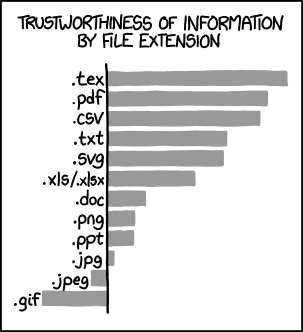
\includegraphics[width=0.47\textwidth]{figs/file_extensions.png}

  % *Every* figure should have a descriptive caption.
%  \caption{On the trustworthiness of \LaTeX. Image courtesy of \texttt{xkcd}.}

  % The label is a handle you create so that you can refer to this
  % figure (using the \ref{} command) from other parts of your
  % document. LaTeX automatically renumbers figures and updates
  % references when you recompile, so you should do it this way rather
  % than hard-coding in references. Notice that I've also been
  % creating labels for the various sections in the document; I could
  % use \ref{} command to refer to those sections using their labels
  % too.
  %\label{fig:tex}

%\end{figure}

%\subsection{Creating Tables}
%\label{subsec:tables}

%Again, refer to \texttt{results.tex} to learn how to create simple
%tables (like table~\ref{tab:example}).


